\documentclass[11pt]{article}
\usepackage{fontspec}
\usepackage{polyglossia}
\setmainlanguage{spanish}
\usepackage[a4paper,margin=2.2cm]{geometry}
\usepackage{amsmath,amssymb}
\usepackage{graphicx}
\usepackage{booktabs}
\usepackage{array}
\usepackage{float}
\usepackage[font=small,labelfont=bf]{caption}
\usepackage{enumitem}
\usepackage{xcolor}
\usepackage[most]{tcolorbox}
\usepackage{tikz}
\usetikzlibrary{arrows.meta,positioning,calc}
\usepackage{hyperref}
\hypersetup{colorlinks=true,linkcolor=azul,urlcolor=azul}
\usepackage{fancyhdr}
\usepackage{titlesec}

\definecolor{azul}{HTML}{1F4E79}
\definecolor{gris}{HTML}{F2F4F7}
\definecolor{rojo}{HTML}{C0504D}

\titleformat{\section}{\large\bfseries\color{azul}}{\thesection.}{0.6em}{}
\titleformat{\subsection}{\normalsize\bfseries\color{azul}}{\thesubsection}{0.6em}{}
\setlength{\parskip}{0.45em}
\setlength{\parindent}{0pt}
\setlist{itemsep=0.15em,topsep=0.3em}

\newtcolorbox{clave}[1][]{colback=gris,colframe=azul,boxrule=0.6pt,arc=2pt,left=6pt,right=6pt,top=4pt,bottom=4pt,fonttitle=\bfseries\small,title={#1}}
\newtcolorbox{alerta}[1][]{colback=rojo!6,colframe=rojo,boxrule=0.6pt,arc=2pt,left=6pt,right=6pt,top=4pt,bottom=4pt,fonttitle=\bfseries\small,title={#1}}

\pagestyle{fancy}
\fancyhf{}
\renewcommand{\headrulewidth}{0.4pt}
\fancyfoot[C]{\small\thepage}

\fancyhead[L]{\small Justificación — Observadores de Luenberger y Kalman en el SCARA}
\fancyhead[R]{\small Universidad EIA}
\newtcolorbox{preg}[1][]{colback=white,colframe=azul!55,boxrule=0.5pt,arc=2pt,left=6pt,right=6pt,top=3pt,bottom=3pt,fonttitle=\bfseries\small,title={#1},breakable}
\newcommand{\cod}[1]{\texttt{#1}}
\usepackage{fancyvrb}

\begin{document}

\begin{center}
{\LARGE\bfseries\color{azul} Justificación de la implementación de los\\[0.15em] observadores de Luenberger y Kalman}\\[0.4em]
{\large Robot SCARA · ESP32 con ESP-IDF · ROS 2 / micro-ROS}\\[0.6em]
{\small Juan David Botero · Universidad EIA · octubre de 2026 · código: \cod{src/estimator.c}, \cod{src/control.c}, \cod{ros2/scara\_panel.py}}
\end{center}

\begin{clave}[Resumen]
\small
\begin{tabular}{@{}>{\raggedright\arraybackslash}p{3.6cm}>{\raggedright\arraybackslash}p{12.1cm}@{}}
Qué estiman & Corriente de armadura (no se mide) y velocidad (se mide con ruido de cuantización) de los 3 motores. \\
Dónde & En el ESP32, a 100 Hz ($T_s=10$ ms), dentro de la tarea de control de 1 kHz. Se publican por \cod{/scara/obs} y se grafican en el panel. \\
Modelo & El del Laboratorio 4 (Pololu 37D 100:1), referido al eje de salida. Discretización exacta (ZOH) calculada en el propio ESP32. \\
Luenberger & Polos $0{,}25\pm0{,}25j$ por Ackermann: $L=[0{,}2436\ \ 0{,}4120]^T$. Converge en 4--5 muestras. \\
Kalman & $R=(0{,}81\ \text{rpm})^2$ medido; $Q=\operatorname{diag}(10\ \text{mA},\ 0{,}30\ \text{rpm})^2$. $K$ converge en 8 muestras a $K_w=0{,}266$. \\
Validación & Mismos $A$, $B$, $L$ y $K$ que el laboratorio; con los datos reales del laboratorio, misma salida que el MATLAB (diferencia máxima $2\times10^{-5}$ rpm). Pruebas automáticas y simulación con encoder cuantizado. \\
\end{tabular}
\end{clave}

%=====================================================================
\section{Para qué se implementaron}

\begin{itemize}
  \item \textbf{La corriente no se mide.} El sensado de corriente de la tarjeta no está activo, y la corriente es la variable que da el par ($\tau=K_v\,i$). Es la base para el control de par del atornillador. Los observadores la reconstruyen a partir de la velocidad y del voltaje aplicado.
  \item \textbf{La velocidad medida es gruesa.} Se obtiene contando pulsos del encoder en 10 ms: llega en escalones de 0,93 rpm. El Kalman la filtra sin el retraso de un filtro pasa bajos común, porque usa el modelo para predecir.
  \item \textbf{Llevar el laboratorio al robot.} El Laboratorio 4 diseñó y probó los observadores fuera de línea (MATLAB y LabVIEW con un motor). Aquí corren en tiempo real, en el microcontrolador del robot, para los tres motores a la vez.
\end{itemize}

%=====================================================================
\section{Del laboratorio al robot: qué se conserva y qué cambia}

\begin{table}[H]\centering\small
\begin{tabular}{>{\raggedright\arraybackslash}p{3.3cm}>{\raggedright\arraybackslash}p{5.4cm}>{\raggedright\arraybackslash}p{6.8cm}}
\toprule
 & Laboratorio 4 & Robot (este trabajo) \\
\midrule
Modelo & $R_a$, $L_a$ medidos; $K_v$, $\beta$, $J$ ajustados & El mismo, \textbf{referido al eje de salida} \\
$T_s$, polos, $Q$, $R$, $P_0$ & 10 ms; $0{,}25\pm0{,}25j$; los de la tabla \ref{tab:qr} & Iguales \\
Diseño & MATLAB, fuera de línea & En el ESP32 (exponencial de matriz y Ackermann), así se puede rediseñar en vivo \\
Ejecución & Formula Node en LabVIEW (myRIO), 1 motor & C en el ESP32, 3 motores, cada 10 ticks del lazo de 1 kHz \\
Driver & L298N ($g=0{,}9782$, $v_0=1{,}197$ V) & TB6612 ($g=1$, $v_0\approx0{,}8$ V), configurable \\
Encoder & 6533 cuentas/vuelta (caja 102,08:1) & 6424 cuentas/vuelta (configuración del robot) \\
Visualización & Gráficas de LabVIEW & Tópico \cod{/scara/obs} y panel PyQt5; CSV \\
\bottomrule
\end{tabular}
\end{table}

\textbf{Por qué referir el modelo al eje de salida.} En el laboratorio el estado tenía $\omega$ del eje del motor y la salida en rpm del eje de salida, con la relación $N$ metida en $C$. En el robot se trabaja con $\omega$ de la articulación en rad/s: $K_v\to K_vN$, $\beta\to\beta N^2$, $J\to JN^2$. Así $C=[0\ \ 1]$, las unidades son las del control de posición y el diseño no depende de si la caja es 100,37:1 o 102,08:1. Las ganancias son las mismas en otras unidades:
\[
L_{lab}=\begin{bmatrix}0{,}02551\ \tfrac{\text{A}}{\text{rpm}}\\ 4{,}4039\ \tfrac{\text{rad/s motor}}{\text{rpm}}\end{bmatrix}
\ \Rightarrow\
L=\begin{bmatrix}0{,}02551/(\pi/30)\\ 4{,}4039/(N\pi/30)\end{bmatrix}=\begin{bmatrix}0{,}2436\\ 0{,}4120\end{bmatrix},\qquad
K_{w}=\frac{2{,}84}{N\,\pi/30}=0{,}266
\]

%=====================================================================
\section{Modelo, entrada y medida}

\subsection*{Modelo}
\begin{equation}
L_a\frac{di}{dt}=V-R_ai-K_v\omega,\qquad J\frac{d\omega}{dt}=K_vi-\beta\omega,\qquad x=\begin{bmatrix}i\\ \omega\end{bmatrix},\ \ y=\omega
\end{equation}
\begin{equation}
A_c=\begin{bmatrix}-R_a/L_a & -K_v/L_a\\ K_v/J & -\beta/J\end{bmatrix}=\begin{bmatrix}-833{,}3 & -2{,}785\\ 460{,}0 & -7{,}687\end{bmatrix},\qquad
B_c=\begin{bmatrix}1/L_a\\ 0\end{bmatrix}=\begin{bmatrix}16{,}67\\ 0\end{bmatrix}
\end{equation}
con $R_a=50~\Omega$, $L_a=0{,}060$ H, $K_v=0{,}167092$ V·s/rad, $\beta=2{,}792\times10^{-3}$ N·m·s/rad y $J=3{,}632\times10^{-4}$ kg·m² (eje de salida). Polos: $-831{,}8$ s$^{-1}$ (eléctrico, 1,2 ms) y $-9{,}24$ s$^{-1}$ (mecánico, 108 ms). A 12 V: 114,30 rpm y 0,2000 A, como se ajustó en el laboratorio.

\subsection*{Entrada: voltaje medio del intervalo}
El observador necesita el voltaje que de verdad recibe el motor. El PWM cambia cada 1 ms (lazo de control), así que en cada intervalo de 10 ms se suma el PWM de los 10 ticks y se usa el promedio:
\begin{equation}
\bar d_{k-1}=\frac{1}{10}\sum_{n=1}^{10} d_n,\qquad u_{k-1}=g\,(12\,\bar d_{k-1})-\operatorname{signo}(\bar d_{k-1})\,v_0\quad(0 \text{ si }|g\,12\,\bar d|<v_0)
\end{equation}
Es lo que exige el modelo discreto: $x_k=Ax_{k-1}+Bu_{k-1}$ supone $u$ constante en el intervalo, y el promedio es el voltaje equivalente. La zona muerta $v_0$ representa la fricción seca: por debajo de ella el motor no se mueve, y sin ella el modelo predeciría movimiento donde no lo hay. $g$ y $v_0$ se cambian en vivo con \cod{vmap g v0}.

\subsection*{Medida: diferencia de cuentas}
\begin{equation}
y_k=\frac{c_k-c_{k-1}}{6424}\cdot\frac{2\pi}{T_s}\quad[\text{rad/s}],\qquad \Delta y=\frac{2\pi}{6424\cdot0{,}01}=0{,}098\ \text{rad/s}=0{,}93\ \text{rpm por cuenta}
\end{equation}
Si fuera solo cuantización, su varianza sería $\Delta^2/12=0{,}073$ rpm². La medida en el laboratorio dio $R=0{,}655$ rpm² ($\sigma_y=0{,}81$ rpm): el encoder real tiene además irregularidad entre pulsos y rizado de par. Por eso se usa el valor \textbf{medido} y no el teórico.

\textbf{Por qué 10 ms y no 1 ms.} En 1 ms una cuenta equivale a 9,3 rpm: la medida sería casi solo ruido. Con 10 ms se conserva además todo el diseño del laboratorio. El PID sigue a 1 kHz con su propia velocidad filtrada; los observadores no están dentro del lazo de control (se usan para monitorear y para el futuro control de par).

%=====================================================================
\section{Discretización exacta}

\begin{equation}
\exp\!\left(\begin{bmatrix}A_c & B_c\\ 0 & 0\end{bmatrix}T_s\right)=\begin{bmatrix}A & B\\ 0 & 1\end{bmatrix},\qquad
A=\begin{bmatrix}-0{,}001479 & -0{,}003086\\ 0{,}50976 & 0{,}91345\end{bmatrix},\quad B=\begin{bmatrix}0{,}019769\\ 0{,}077830\end{bmatrix}
\end{equation}
\begin{itemize}
  \item \textbf{ZOH es exacto aquí}, porque el driver mantiene el voltaje (el promedio) constante durante el intervalo.
  \item \textbf{Euler no sirve:} el polo eléctrico daría $1+\lambda T_s=1-831{,}8\cdot0{,}01=-7{,}3$, fuera del círculo unitario. El modelo discreto sería inestable y el observador divergería.
  \item \textbf{Cómo se calcula en el ESP32} (\cod{expm3}): la matriz 3×3 se divide por $2^s$ hasta que su norma sea menor que 0,25, se suma la serie de Taylor hasta el término 14 y se eleva al cuadrado $s$ veces. Se hace en \cod{double} y solo al diseñar (al arrancar o con \cod{luen}/\cod{kal}), no en cada muestra. Coincide con \cod{expm} de MATLAB/scipy en todas las cifras mostradas.
  \item \textbf{Lectura física:} $A_{11}\approx0$ porque la corriente se estabiliza en 1,2 ms, mucho antes de los 10 ms del período. El polo mecánico discreto es $e^{-9{,}24\cdot0{,}01}=0{,}912$.
\end{itemize}

%=====================================================================
\section{Observabilidad}
Con $C=[0\ \ 1]$:
\begin{equation}
\mathcal O=\begin{bmatrix}C\\ CA\end{bmatrix}=\begin{bmatrix}0 & 1\\ 0{,}5098 & 0{,}9135\end{bmatrix},\qquad \det\mathcal O=-A_{21}=-0{,}51\neq0\ \Rightarrow\ \operatorname{rango}\mathcal O=2
\end{equation}
El sistema es observable si y solo si $A_{21}\neq0$: la corriente produce par y el par cambia la velocidad. El firmware revisa esa condición al diseñar (\cod{observable = |A21| > 1e-9}).

%=====================================================================
\section{Observador de Luenberger}

\subsection*{Forma}
Se usa la forma \emph{predictor} de la guía: el estado en $k$ se calcula con la medida y la entrada de $k-1$.
\begin{equation}
\hat x_k=A\hat x_{k-1}+Bu_{k-1}+L\,(y_{k-1}-C\hat x_{k-1}),\qquad e_k=x_k-\hat x_k=(A-LC)\,e_{k-1}
\end{equation}
El error decae con los polos de $A-LC$, que se eligen libremente porque el sistema es observable.

\subsection*{Ganancia por Ackermann}
\begin{equation}
L=\Phi(A)\,\mathcal O^{-1}\begin{bmatrix}0\\1\end{bmatrix},\qquad \Phi(z)=(z-p_1)(z-p_2)=z^2-2\,\mathrm{Re}(p)\,z+|p|^2
\end{equation}
Con $C=[0\ \ 1]$, $\mathcal O^{-1}[0\ \ 1]^T=[1/A_{21}\ \ 0]^T$, y la fórmula se reduce a
\begin{equation}
L=\frac{1}{A_{21}}\begin{bmatrix}\Phi(A)_{11}\\ \Phi(A)_{21}\end{bmatrix}
\end{equation}
que es lo que calcula el firmware (dos productos y una división, sin invertir matrices). Con $p=0{,}25\pm0{,}25j$: $\Phi(A)=A^2-0{,}5A+0{,}125I$, y
\[
L=\begin{bmatrix}0{,}2436\ \ \text{A por rad/s}\\ 0{,}4120\end{bmatrix},\qquad \operatorname{eig}(A-LC)=0{,}25\pm0{,}25j\ \ \text{(verificado)}
\]

\subsection*{Elección de los polos}
$|p|=0{,}354$, constante de tiempo $-T_s/\ln|p|=9{,}6$ ms: unas 10 veces más rápido que el polo mecánico (0,912). Se compararon otras ubicaciones en las mismas condiciones del robot (planta identificada, zona muerta, encoder cuantizado a 10 ms, escalones de PWM):

\begin{table}[H]\centering\small
\begin{tabular}{lccc>{\raggedright\arraybackslash}p{5.2cm}}
\toprule
Polos & $L$ & Error vel. [rpm] & Ruido corriente [mA] & Lectura \\
\midrule
$0{,}05$ (doble) & $[0{,}002;\ 0{,}81]$ & 0,33 & 0,3 & casi \emph{deadbeat}: copia la medida y su ruido en velocidad; corriente limpia \\
$\mathbf{0{,}25\pm0{,}25j}$ & $[0{,}244;\ 0{,}41]$ & \textbf{0,13} & 13,4 & equilibrio; los del laboratorio \\
$0{,}5$ (doble) & $[0{,}490;\ -0{,}09]$ & 0,09 & 20,5 & velocidad más suave, corriente más ruidosa \\
$0{,}7$ (doble) & $[0{,}962;\ -0{,}49]$ & 0,17 & 33,1 & cerca de la planta: peor en todo \\
$0{,}85$ (doble) & $[1{,}419;\ -0{,}79]$ & 0,25 & 50,4 & más lento que el propio modelo \\
\bottomrule
\end{tabular}
\caption{Estudio de polos en simulación (error RMS en los tramos estables; medida sin filtrar: 0,40 rpm). En el laboratorio, con los datos reales, $0{,}25\pm0{,}25j$ dio el menor error de velocidad (0,67 rpm).}
\end{table}
La decisión: $0{,}25\pm0{,}25j$, porque converge en pocas muestras, reduce el error de velocidad a la tercera parte de la medida y fue la mejor opción con datos reales en el laboratorio. Su precio es que deja pasar ruido a la corriente; para eso está el Kalman. Se pueden cambiar en vivo con \cod{luen j re im} (se rechazan polos con $|p|\ge1$).

%=====================================================================
\section{Filtro de Kalman}

\subsection*{Forma}
Se usa la forma de estimador actual: predice con $u_{k-1}$ y corrige con la medida de \emph{este} instante, $y_k$.
\begin{align}
\text{a priori:}\quad & \hat x^-_k=A\hat x_{k-1}+Bu_{k-1}, & P^-_k&=AP_{k-1}A^T+Q\\
\text{ganancia:}\quad & K_k=\frac{P^-_kC^T}{CP^-_kC^T+R}=\frac{1}{P^-_{22}+R}\begin{bmatrix}P^-_{12}\\ P^-_{22}\end{bmatrix} & &\\
\text{a posteriori:}\quad & \hat x_k=\hat x^-_k+K_k\,(y_k-\hat x^-_{k,2}), & P_k&=(I-K_kC)\,P^-_k
\end{align}
Con $C=[0\ \ 1]$ la ``inversa'' es una división escalar: no hay inversión de matrices en el microcontrolador.

\subsection*{Covarianzas}
\begin{table}[H]\centering\small
\begin{tabular}{@{}lll>{\raggedright\arraybackslash}p{3.1cm}>{\raggedright\arraybackslash}p{4.4cm}@{}}
\toprule
 & Laboratorio & Robot (eje de salida) & Firmware & De dónde sale \\
\midrule
$R$ & 0,655 rpm² & $(0{,}0848\ \text{rad/s})^2$ & \cod{OBS\_SIG\_Y\_RPM} = 0,81 & varianza de la velocidad medida a velocidad constante \\
$Q_{11}$ & $10^{-4}$ A² & $(0{,}010\ \text{A})^2$ & \cod{OBS\_SIG\_I} = 0,010 & cuánto se desconfía del modelo en la corriente \\
$Q_{22}$ & 10,28 (rad/s motor)² & $(0{,}0314\ \text{rad/s})^2$ & \cod{OBS\_SIG\_W\_RPM} = 0,30 & cuánto se desconfía del modelo en la velocidad \\
$P_0$ & diag(0,01; 114,3) & diag$(0{,}1\ \text{A};\ 1\ \text{rpm})^2$ & \cod{OBS\_P0\_*} & incertidumbre inicial \\
\bottomrule
\end{tabular}
\caption{Matrices del Kalman (mismos valores, en las unidades de cada implementación).}
\label{tab:qr}
\end{table}
En el primer paso se toma $\hat x=0$ y $P=P_0$ sin corregir, igual que el código de MATLAB, para que la secuencia sea idéntica.

\subsection*{Convergencia y valor estable}
$K_w$ toma los valores 0,639; 0,402; 0,322; 0,290; \dots\ y queda a menos del 1 \% de su valor final en 8 muestras (80 ms):
\[
K_{ss}=\begin{bmatrix}-5{,}57\times10^{-4}\ \ \text{A por rad/s}\\ 0{,}266\end{bmatrix},\qquad \sqrt{P_{\omega}}=0{,}42\ \text{rpm},\qquad \sqrt{P_i}=10\ \text{mA}
\]
Se calcula en línea en vez de usar $K_{ss}$ fija: cuesta unas 30 multiplicaciones por motor cada 10 ms, permite ver en el panel cómo convergen $P$ y $K$ (lo que pide el laboratorio) y permite cambiar $Q$ y $R$ en vivo con \cod{kal j sig\_i sig\_w sig\_y}.

\subsection*{Por qué $K_i\approx0$}
Las mismas dos razones del laboratorio, ambas del modelo y no del filtro: con $R_a=50~\Omega$ la corriente la fija casi solo el voltaje aplicado ($i\approx(V-K_v\omega)/R_a$, y $K_v\omega$ es como mucho 2 V), y la dinámica eléctrica (1,2 ms) es mucho más rápida que $T_s$. La velocidad trae muy poca información nueva sobre la corriente, así que el filtro casi no la corrige: la corriente sale del modelo y por eso no tiene ruido.

\subsection*{Sensibilidad a $Q$ y $R$}
\begin{table}[H]\centering\small
\begin{tabular}{>{\raggedright\arraybackslash}p{4.3cm}ccc>{\raggedright\arraybackslash}p{3.6cm}}
\toprule
Cambio & $K_w$ & Error vel. & Ruido corr. & Efecto \\
 & & [rpm] & [mA] & \\
\midrule
Diseño: $\sigma_i$ 10 mA, $\sigma_\omega$ 0,30 rpm, $\sigma_y$ 0,81 rpm & 0,266 & 0,092 & 0,02 & — \\
$\sigma_i$ = 1 mA / 100 mA & 0,262 / 0,471 & 0,091 / 0,161 & 0,02 / 0,04 & poco efecto \\
$\sigma_\omega$ = 0,10 rpm & 0,075 & 0,049 & 0,02 & más confianza en el modelo \\
$\sigma_\omega$ = 1,0 rpm & 0,677 & 0,247 & 0,05 & más confianza en la medida \\
$\sigma_y$ = 0,27 rpm (solo cuantización) & 0,643 & 0,232 & 0,05 & sigue más a la medida \\
\bottomrule
\end{tabular}
\caption{En simulación con la planta exacta, bajar $Q$ siempre ``mejora''. En el robot no: ver la sección \ref{sec:robustez}.}
\end{table}

%=====================================================================
\section{Implementación en el firmware}

\begin{figure}[H]\centering
\begin{tikzpicture}[font=\scriptsize, node distance=5mm,
  caja/.style={draw=azul, rounded corners=2pt, fill=gris, align=center, inner sep=3pt, text width=2.2cm},
  flecha/.style={-{Stealth[length=1.8mm]}, thick, azul}]
\node[caja] (pcnt) {Encoder (PCNT)\\ cuentas $c$};
\node[caja, below=of pcnt] (pwm) {PWM de cada tick\\ (lazo 1 kHz)};
\node[caja, right=6mm of pcnt] (y) {velocidad medida\\ $y_k$: cuentas en 10 ms};
\node[caja, right=6mm of pwm] (u) {promedio de 10 ticks\\ $u=g\,12\,\bar d-v_0$};
\node[caja, text width=2.4cm] (est) at ($(y.east)!0.5!(u.east)+(2.0cm,0)$) {\cod{est\_step()}\\ Luenberger + Kalman\\ cada 10 ticks (100 Hz)};
\node[caja, right=6mm of est, text width=1.9cm] (snap) {copia protegida\\ (sección crítica)};
\node[caja, right=6mm of snap, text width=1.8cm] (pub) {\cod{/scara/obs}\\ 20 Hz\\ panel y CSV};
\draw[flecha] (pcnt) -- (y); \draw[flecha] (pwm) -- (u);
\draw[flecha] (y) -- (est); \draw[flecha] (u) -- (est);
\draw[flecha] (est) -- (snap); \draw[flecha] (snap) -- (pub);
\end{tikzpicture}
\caption{Flujo de datos de los observadores en el ESP32.}
\end{figure}

\begin{itemize}
  \item \textbf{Dónde corre.} En la misma tarea del lazo de control (1 kHz): cada 10 ticks llama a \cod{observadores()}. Así la medida y el voltaje medio corresponden exactamente al mismo intervalo de 10 ms, sin desfase entre tareas.
  \item \textbf{Costo.} Por motor y por muestra: unas 6 multiplicaciones el Luenberger y unas 30 el Kalman, en \cod{float} (el ESP32 tiene unidad de punto flotante). Para 3 motores a 100 Hz es una fracción mínima del tiempo de CPU; el diseño (exponencial, Ackermann) se hace en \cod{double} y solo al cambiar parámetros.
  \item \textbf{Publicación.} El resultado se copia dentro de una sección crítica a un búfer; la tarea de micro-ROS lo publica a 20 Hz. El panel ve una de cada 5 muestras (el observador sigue corriendo a 100 Hz). El paquete lleva un número de secuencia para detectar pérdidas.
  \item \textbf{Validez del diseño.} \cod{est\_design} devuelve \cod{ok = false} si el sistema no es observable o algún polo tiene $|p|\ge1$; un \cod{luen} inválido se rechaza con un mensaje y se conserva el diseño anterior.
  \item \textbf{Motor sin encoder} (M3 si \cod{M3\_TIENE\_ENCODER 0}): corre solo con el modelo, sin corrección ($K=0$, $P$ crece con $Q$). A 12 V da 0,2 A y 114,3 rpm, como el modelo.
  \item \textbf{Comandos en vivo} (panel, \cod{/scara/cmd} o monitor serie): \cod{est j} muestra el diseño, \cod{est reset} reinicia ($\hat x=0$, $P=P_0$), \cod{luen j re im}, \cod{kal j mA rpm rpm}, \cod{vmap g v0}.
\end{itemize}

\textbf{Núcleo del paso (extracto de \cod{src/estimator.c})}
\begin{Verbatim}[fontsize=\footnotesize, frame=single, rulecolor=\color{azul!50}]
/* Luenberger (predictor): medida y entrada de k-1 */
inn      = y_prev - xl[1];                         /* y(k-1) - C x^(k-1)   */
xl[0]    = A00*x0 + A01*x1 + B0*u_prev + L0*inn;
xl[1]    = A10*x0 + A11*x1 + B1*u_prev + L1*inn;
/* Kalman: predicción */
xp       = A*xk + B*u_prev;                        /* a priori             */
Pm       = A*Pk*A' + diag(sig_i^2, sig_w^2);
/* Kalman: corrección con y(k) (C = [0 1]: una división) */
S        = Pm[1][1] + sig_y^2;
K        = { Pm[0][1]/S, Pm[1][1]/S };
xk       = xp + K*(y - xp[1]);                     /* a posteriori         */
Pk       = (I - K*C)*Pm;
\end{Verbatim}

\textbf{Qué viaja por \cod{/scara/obs}} (por motor, 12 datos): velocidad medida, Luenberger, Kalman a priori, Kalman a posteriori [rpm]; corriente Luenberger, Kalman a priori, Kalman a posteriori [A]; $\sqrt{P_i}$ [A], $\sqrt{P_\omega}$ [rpm]; $K_w$, $K_i$; voltaje del modelo [V]. Son exactamente las curvas que pide el laboratorio: velocidad y corriente de cada observador, a priori y a posteriori, y el comportamiento de $P$ y $K$.

%=====================================================================
\section{Validación}

\begin{enumerate}
  \item \textbf{Diseño.} La prueba \cod{test\_estimator.c} comprueba que el C da los mismos $A$, $B$, $L$ (Ackermann) y $K_{ss}$ que el laboratorio, y que los polos de $A-LC$ son los pedidos.
  \item \textbf{Contra MATLAB con datos reales.} Con la secuencia de PWM y las velocidades medidas en el laboratorio, la salida del C coincide con la del MATLAB con una diferencia máxima de $2\times10^{-5}$ rpm (precisión de \cod{float}).
  \item \textbf{Copia en Python.} El modo demo del panel usa una copia en Python (\cod{scara\_common.Estimator}) que da los mismos números; también se prueba.
  \item \textbf{Simulación con encoder cuantizado} (figuras \ref{fig:obs} y \ref{fig:conv}): error RMS de velocidad 0,40 rpm la medida, 0,13 el Luenberger y 0,09 el Kalman; ruido de corriente 13 mA el Luenberger y prácticamente nulo el Kalman. Tras un reinicio con el motor a 72 rpm, el Luenberger vuelve a menos de 1 rpm en 5 muestras y el Kalman en 9; la corriente del Kalman es correcta desde la primera muestra porque sale del voltaje.
  \item \textbf{En el robot:} firmware cargado en el ESP32 y observadores visibles en el panel.
\end{enumerate}

\begin{figure}[H]\centering
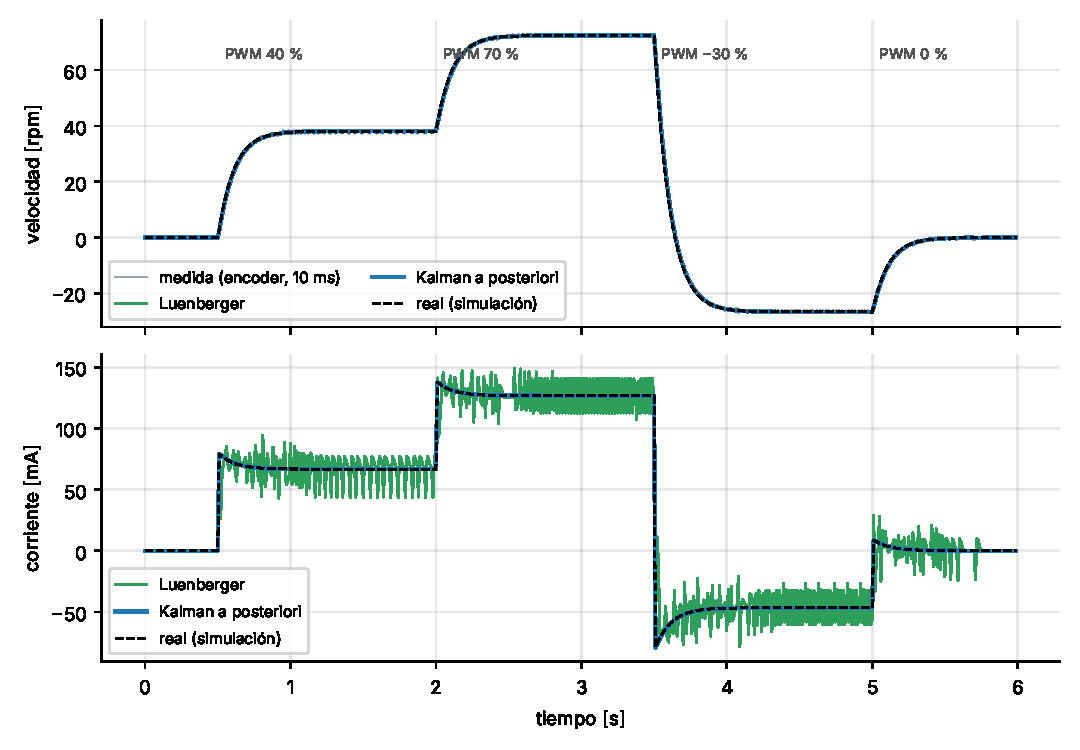
\includegraphics[width=0.9\linewidth]{figs/f_observadores.pdf}
\caption{Simulación con la planta identificada, zona muerta de 0,8 V y encoder de 6424 cuentas leído cada 10 ms. En velocidad las curvas casi coinciden; en corriente el Luenberger deja pasar el ruido de cuantización.}
\label{fig:obs}
\end{figure}

\begin{figure}[H]\centering
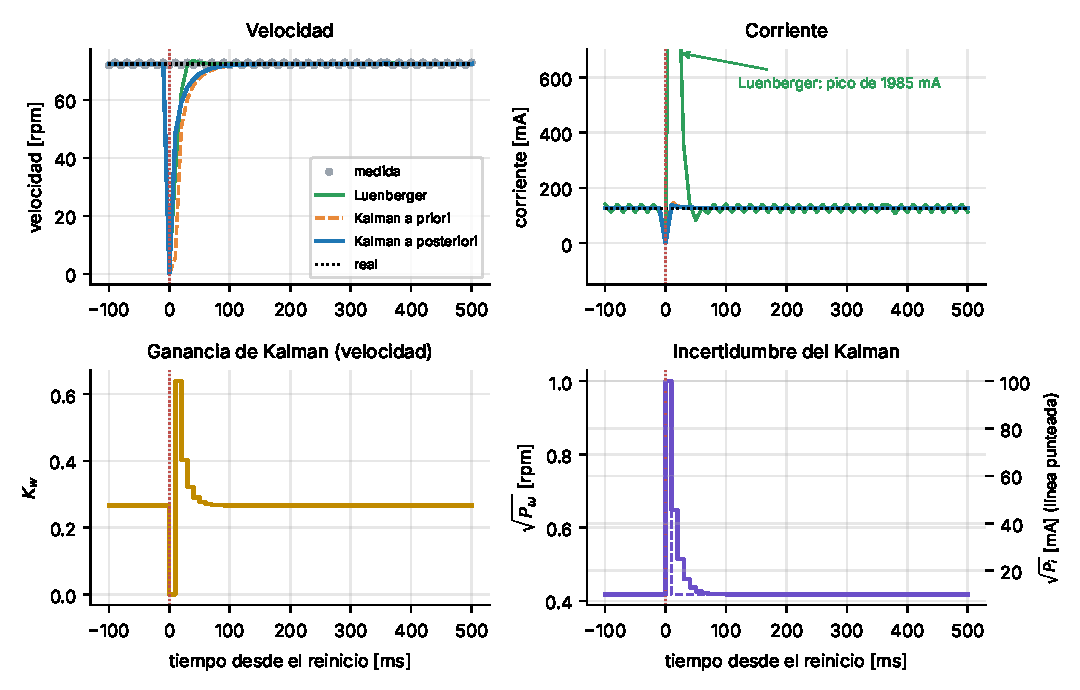
\includegraphics[width=0.9\linewidth]{figs/f_convergencia.pdf}
\caption{Botón \emph{Reiniciar observadores} con el motor a 70 \% (72 rpm, 127 mA): $\hat x=0$ y $P=P_0$. El Luenberger corrige más rápido la velocidad pero su $L$ grande produce un pico de corriente; el Kalman arranca con $K$ alta (0,64) porque $P_0$ es grande y la baja a 0,266 a medida que $P$ converge.}
\label{fig:conv}
\end{figure}

%=====================================================================
\section{Robustez y limitaciones}\label{sec:robustez}

En la simulación el Kalman conoce la planta exacta. En el robot no: el eslabón cambia la inercia, hay fricción que el modelo no tiene y $R_a$ puede no ser 50~$\Omega$. Se simuló el filtro con una planta distinta al modelo:

\begin{table}[H]\centering\small
\begin{tabular}{lccccc}
\toprule
Planta real & $\sigma_\omega$ & Medida & Luenberger & Kalman & Sesgo corriente Kalman \\
 & [rpm] & \multicolumn{3}{c}{error RMS de velocidad [rpm]} & [mA] \\
\midrule
$J$ +50 \% (eslabón) & 0,30 & 0,42 & 0,15 & 0,17 & 0,0 \\
Fricción seca extra (= 0,5 V) & 0,30 & 0,44 & 0,68 & \textbf{0,94} & $-0{,}1$ \\
Fricción seca extra (= 0,5 V) & 1,0 & 0,44 & 0,68 & \textbf{0,32} & 0,0 \\
$R_a$ real = 40 $\Omega$ & 0,30 & 0,30 & 1,45 & \textbf{2,00} & $-11$ \\
$R_a$ real = 40 $\Omega$ & 1,0 & 0,30 & 1,45 & \textbf{0,47} & $-11$ \\
\bottomrule
\end{tabular}
\caption{Con un modelo equivocado y $Q$ pequeño, el Kalman confía demasiado en el modelo y su velocidad se aleja de la medida. Subir $\sigma_\omega$ a 1 rpm lo corrige. El sesgo de corriente por un $R_a$ equivocado no lo arregla $Q$: es del modelo.}
\end{table}

\begin{alerta}[Limitaciones que hay que decir]
\begin{itemize}
  \item \textbf{La corriente estimada depende del modelo.} Con $R_a=50~\Omega$ (alto para este motor: la hoja de datos sugiere unos 2,2~$\Omega$) el modelo da poco par por amperio. Sirve para ver tendencias; para usarla como medida hay que validarla con un amperímetro o con la corriente de la fuente ($I_{fuente}\approx I_{lógica}+\sum|i|\,d$, que el panel calcula).
  \item \textbf{Si en el robot la velocidad del Kalman queda corrida respecto a la medida} en régimen permanente, el modelo no coincide con ese eje: subir $\sigma_\omega$ (\cod{kal j 10 1.0 0.81}) o ajustar $v_0$ con \cod{vmap}.
  \item \textbf{El modelo se identificó con el motor solo y un L298N}; el robot usa un TB6612 y tiene eslabones. $v_0=0{,}8$ V es una estimación.
  \item \textbf{La medida es un promedio de 10 ms}, no la velocidad instantánea (medio período de retraso). Es la misma convención del laboratorio.
\end{itemize}
\end{alerta}

%=====================================================================
\section{Cómo mostrarlo en la presentación}

\begin{enumerate}
  \item Panel, pestaña \textbf{Observadores}, elegir M1. Modo \textbf{Potencia}, M1 a 30--50 \%, mantener el dead-man: se ven la velocidad medida (escalonada), Luenberger y Kalman a priori y a posteriori, y las dos corrientes.
  \item Señalar la corriente: la del Luenberger con ruido, la del Kalman limpia. Explicar por qué (secciones 6 y 7).
  \item Con el motor girando, pulsar \textbf{Reiniciar observadores} (tecla \cod{r}): se ve la convergencia, el salto de $K_w$ a 0,64 y su bajada a 0,266, y cómo $\sqrt P$ baja.
  \item En \textbf{Sintonía}: poner polo re = 0,05 e im = 0 y \emph{Aplicar Luenberger} (la corriente se limpia y la velocidad se vuelve más escalonada); volver a 0,25. Subir $\sigma_\omega$ a 1 rpm en el Kalman: $K_w$ sube a 0,68 y la velocidad sigue más a la medida.
  \item Pestaña \textbf{Motores}: corriente estimada de los 3 motores y la de la fuente estimada para comparar con el amperímetro.
  \item \textbf{Grabar CSV} durante la prueba para tener los datos y graficarlos en MATLAB si lo piden.
\end{enumerate}

%=====================================================================
\section{Preguntas probables y respuestas}

\begin{preg}[1. ¿Para qué observadores si el encoder ya mide la velocidad?]
La corriente no se mide y es la que da el par; los observadores la estiman. Y la velocidad del encoder llega en escalones de 0,93 rpm: el Kalman la filtra usando el modelo, sin el retraso de un filtro pasa bajos.
\end{preg}

\begin{preg}[2. ¿Cómo saben que se puede estimar la corriente midiendo solo la velocidad?]
Observabilidad: $\det[C;\,CA]=-A_{21}=-0{,}51\neq0$, rango 2. La corriente produce par y el par cambia la velocidad.
\end{preg}

\begin{preg}[3. ¿Por qué 10 ms si el control corre a 1 kHz?]
Una cuenta del encoder en 1 ms son 9,3 rpm; en 10 ms, 0,93 rpm. Además así se conservan $T_s$, $R$ y los polos del laboratorio. Los observadores no están dentro del lazo del PID.
\end{preg}

\begin{preg}[4. ¿Por qué discretizaron con la exponencial de matriz?]
Porque ZOH es exacto para voltaje constante en el intervalo. Euler con $T_s=10$ ms pondría el polo eléctrico en $-7{,}3$, inestable. Se calcula en el ESP32 para poder rediseñar sin MATLAB.
\end{preg}

\begin{preg}[5. ¿Qué voltaje le dan al observador si el PWM cambia cada 1 ms?]
El promedio de los 10 PWM del intervalo, convertido a voltaje con la ganancia del driver y la zona muerta. Es el voltaje constante equivalente que supone el modelo discreto.
\end{preg}

\begin{preg}[6. ¿Cómo calcularon L?]
Ackermann: $L=\Phi(A)\,\mathcal O^{-1}[0\ 1]^T$. Con $C=[0\ 1]$ se reduce a la primera columna de $\Phi(A)$ dividida por $A_{21}$. Da $[0{,}2436\ \ 0{,}4120]^T$, lo mismo que el laboratorio en otras unidades, y los polos de $A-LC$ quedan en $0{,}25\pm0{,}25j$.
\end{preg}

\begin{preg}[7. ¿Por qué esos polos?]
$|p|=0{,}35$: converge en 4--5 muestras, 10 veces más rápido que la planta, y reduce el error de velocidad a un tercio del de la medida. Polos más rápidos copian el ruido de la medida; más lentos que la planta empeoran todo. En el laboratorio fueron los de menor error con datos reales.
\end{preg}

\begin{preg}[8. ¿Por qué la corriente del Luenberger es ruidosa?]
Porque $L$ es fija y grande en la corriente ($L_1=0{,}24$ A por rad/s): cada salto de una cuenta del encoder (0,098 rad/s) mueve la corriente estimada unos 24 mA.
\end{preg}

\begin{preg}[9. ¿Qué diferencia hay entre el Luenberger y el Kalman?]
El Luenberger tiene una ganancia fija elegida por polos y no considera el ruido. El Kalman calcula la ganancia que minimiza la varianza del error a partir de cuánto se confía en el modelo ($Q$) y en la medida ($R$). Además el Luenberger usa la medida de $k-1$ (predictor) y el Kalman la de $k$.
\end{preg}

\begin{preg}[10. ¿Qué es a priori y a posteriori?]
A priori: lo que predice el modelo antes de ver la medida, $\hat x^-=A\hat x+Bu$. A posteriori: esa predicción corregida con la medida, $\hat x=\hat x^-+K(y-C\hat x^-)$.
\end{preg}

\begin{preg}[11. ¿De dónde sale R? ¿Por qué no es la varianza de cuantización?]
Se midió en el laboratorio: varianza de la velocidad a velocidad constante, 0,655 rpm². La cuantización sola daría 0,073 rpm²; el resto es irregularidad del encoder y rizado de par. Se usa la medida porque describe el sensor real.
\end{preg}

\begin{preg}[12. ¿Y Q?]
Expresa cuánto se desconfía del modelo: 10 mA en corriente y 0,30 rpm en velocidad, los del laboratorio. Más $Q$: filtro más rápido y más ruidoso; menos $Q$: más suave pero más dependiente de que el modelo sea correcto.
\end{preg}

\begin{preg}[13. ¿Por qué el Kalman casi no corrige la corriente ($K_i\approx0$)?]
Porque con $R_a=50~\Omega$ la corriente la fija el voltaje y la dinámica eléctrica (1,2 ms) es mucho más rápida que $T_s$: la velocidad casi no trae información nueva sobre la corriente. Por eso la corriente del Kalman sale del modelo y no tiene ruido.
\end{preg}

\begin{preg}[14. ¿La ganancia de Kalman es constante?]
No al principio: parte de $P_0$ y en 8 muestras queda en $K_w=0{,}266$. Después es prácticamente constante. Se calcula en línea para mostrar esa convergencia y poder cambiar $Q$ y $R$ en vivo.
\end{preg}

\begin{preg}[15. ¿Qué pasa si el modelo está mal?]
El Luenberger sigue a la medida con su ganancia fija. El Kalman con $Q$ pequeño confía en el modelo y su velocidad se corre; se corrige subiendo $\sigma_\omega$ (en simulación, de 0,94 a 0,32 rpm con fricción no modelada). Un $R_a$ equivocado sesga la corriente y eso no lo arregla $Q$.
\end{preg}

\begin{preg}[16. ¿Cómo validaron que el código del ESP32 está bien?]
Con los mismos datos reales del laboratorio da la misma salida que el MATLAB (diferencia máxima $2\times10^{-5}$ rpm), y las pruebas automáticas comprueban $A$, $B$, $L$, $K$ y los polos.
\end{preg}

\begin{preg}[17. ¿Cuánto procesamiento consume?]
Unas 36 multiplicaciones por motor cada 10 ms, en \cod{float} con la unidad de punto flotante del ESP32: una fracción mínima del tiempo de CPU. Lo costoso (la exponencial) solo se hace al cambiar parámetros.
\end{preg}

\begin{preg}[18. ¿Por qué la corriente estimada no coincide con la de la fuente?]
La fuente suma la parte lógica (ESP32, reguladores, encoders) y, con PWM, solo ve la corriente del motor el tiempo encendido: $I_{fuente}\approx I_{lógica}+\sum|i|\,d$. El resto de la diferencia es el modelo ($R_a$).
\end{preg}

\begin{preg}[19. ¿Qué pasa con un motor sin encoder?]
El observador corre solo con el modelo: no hay corrección ($K=0$) y la incertidumbre $P$ crece. Es útil para ver qué predice el modelo, pero no se corrige.
\end{preg}

\begin{preg}[20. ¿Para qué sirve esto en el robot?]
Para monitorear cada motor (si se frena, si se carga) y como base del control de par del atornillador: $\tau=K_v\,i$ con $K_v=0{,}167$ N·m/A, limitando la corriente estimada. Antes hay que validar la corriente con un amperímetro.
\end{preg}

\end{document}
